\chapter{Object detection}\label{chap:objdet}
\epigraph{All models are wrong, but some are useful.}{George E. P. Box\\\textit{British statistician}}

This chapter investigates the first phase of the translation from the physical world to cyberspace, by evaluating two object detection models from the autonomous driving research domain.  The PointPillar and the CenterPoint model are evaluated for their suitability to automatically create a digital representation of the rail environment. This evaluation is used to answer RQ1. Based on a custom, open dataset, these two models are evaluated to detect masts, tension rods, signals, and relay cabinets. This dataset is one of the contributions of this thesis. Furthermore, this chapter aided in defining the gap identification contribution. A mean Average Precision (\textit{mAP@0.5}) of 70.6\% is achieved. A unique result of this research is the in-depth analysis of the locational error. This analysis shows that the locational accuracy is not yet sufficient for engineering applications and that largest contribution to this error originates from the random error. Furthermore, this chapter shows that transfer learning is an effective solution to reduce the labelling burden. As an example, when using 25\% of the training data the AP for the tension rod class jumps from 9.5\% (no transfer learning) to 70.8\% (with transfer learning). 

\clearpage
\newcommand{\xyplane}{$xy$-plane}

% CaRS: Create a Research Space: https://uwaterloo.ca/writing-and-communication-centre/cars-model-create-research-space
\section{Introduction}
% Move 1: Establish a Research Territory
Climate change due to increased greenhouse gas emissions is having a serious impact on the world~\cite{Easterling2000}. To reduce greenhouse gas emissions of the transport sector, rail transport can play an important role~\cite{e7rail}. The European Union states that by shifting from road transport to rail transport, a significant reduction of greenhouse emissions can be achieved~\cite{term20}.

With the envisioned increase of passenger and freight rail traffic in the near future, there will also be an increased burden on the railway infrastructure. To ensure continued reliability, availability, maintainability and safety of the railway network in an efficient way, it is vital to have an accurate and up-to-date digital representation of the railway environment. These as-is representations can for instance be used for planning work, immersive visualisations, monitoring the infrastructural health, automated inventory assessment, and predictive maintenance. 

Automated creation of these as-is models is challenging because railway environments pose a complex scene structure and span several thousand of kilometres. Scenes contain both discrete objects such as signals, catenary arches, and relay cabinets on the one hand. On the other hand there are continuous objects such as overhead catenary wires and rail tracks. The number of distinct object classes around the track, and the representational diversity within these object classes can both be extremely large, especially for countries with a dense rail network and a long history of rail infrastructure such as the Netherlands.

An appropriate data source to create these as-is models are point clouds. Point clouds are collected by using a laser scanner, which uses the time-of-flight of light pulses to determine the distance between sensor and object. Point clouds can be captured regardless of external illumination variations and provide immediate, precise 3D geometric information.

% Move 2: Establish a Niche
A research area which is well established with regard to scene understanding from point cloud data is the area of autonomous driving vehicles. Typically autonomous driving vehicles are equipped, amongst a plethora of other sensors, with laser scanners. The data from these laser scanners are used to detect other road users such as other vehicles, pedestrians or cyclists. This study aims to leverage the knowledge developed for this domain and evaluate its usability towards the object detection task within railway environments.

% Move 3: Occupy the Niche
Recent surveys on monitoring critical infrastructure using point cloud data reveal that most approaches do not make use of deep learning techniques~\cite{Sharifisoraki23, dekker23}. Instead most approaches still rely heavily on heuristic methods. A downside of heuristic approaches is that they require many hand crafted features and manually tuned parameters. The aim of this research is to bridge this gap by evaluating the usability of deep learning based object detection for the rail domain. Furthermore, it evaluates the locational accuracy of deep-learning based object detection models. Locational accuracy is a factor which is commonly overlooked or ignored by other publications within the rail domain. Most likely, because it is very difficult to obtain ground truth data for the locations of objects. Nonetheless, it is crucial to have accurate locational data when planning construction or using automated construction robots. It is estimated that the required locational accuracy for the majority of engineering applications is around $\pm$5~cm~\footnote{Based on personal communications with Strukton Rail engineers}.

The remainder of this article is organised as follows: First the related work is presented, thereafter the custom dataset is presented together with the pre-processing steps required to prepare the data for ingestion by the machine learning models. This is followed by the methodology, which describes how the models are trained and evaluation. This section also describes how the effectiveness of transfer learning is evaluated and how the locational error is analysed. The results section presents the findings and also details two approaches which had negative findings. The conclusions together with the recommendations are presented at the end of this article.

\section{Related work}
This section will focus on automated methods to derive information from point cloud data to construct an as-is model of the railway infrastructure. Most related work focuses on single tasks such as detecting either the tracks or components of the overhead line equipment such as the catenary wires.

The work by Zhu and Hyyppa~\cite{zhu2014the} use both Airborne Laser Scanning (ALS) and Mobile Laser Scanning (MLS) data for modelling the railway environment in 3D. Their approach is non-supervised and makes use of a large variety of parametric models which are fine tuned for each of the elements of interest. The scene is decomposed into the following elements: ground, trees, buildings, catenary arches, and overhead power lines. Their approach towards modelling buildings is noteworthy, the facades of buildings are extracted from the MLS data and the roofs are extracted from the ALS data.

Pastucha~\cite{pastucha2016catenary} and Arastounia~\cite{arastounia2015automated} both present very similar results, though the work of Arastounia has a higher level of detail. Both works make use of parametric models to detect the tracks and the overhead components. The work of Arastounia focuses on a stretch of 550~m of Austrian railway track, their results are optimised for this stretch, leading to very high accuracy metrics. The work of Pastucha evaluated around 90~km of Polish railway track, detecting over 97\% of support structures.

The work of \citeauthor{cheng2019automatic} focuses on a very specific use case of creating an as-is Building Information Model (BIM) of single-track railway tunnels based on Terrestrial Laser Scanner (TLS) data~\cite{cheng2019automatic}. To obtain a BIM, the authors make heavy use of parametric models. The resulting model has a high accuracy, in the range of mm~--~cm.

\citeauthor{wolf2021asset} also aim at automatically detecting railway assets from point cloud data~\cite{wolf2021asset}. Their approach to detect railway assets from point cloud data is to first render a grey scale image from a slice of point cloud data. The pixel values are the intensity values from the original point cloud data. These slices are taken perpendicular to the rail track. The work shows results of both object detection, based on the YOLOv3 model~\cite{yolov3}, and on semantic segmentation, based on the U-Net~\cite{unet} model. An image based approach has two major benefits; the field of image processing has advanced much further than point based methods and the processing of raster data can be done much more efficient compared to point data. It should be noted that their work is still in a very premature state.

Commonly, before any modelling steps are undertaken, there is some form or pre-processing involved. In general the goal of this step is to cull the number of points, which is done to lessen the computation load. Often, this step also partitions a large scene into smaller tractable pieces.

Usually when collecting data of the rail environment, also the trajectory of the measurement train is logged. This trajectory is a valuable resource when partitioning the large point cloud scene into smaller tractable pieces. A trajectory log based dissection method is described by \citeauthor{soilan2021fully}. Their method~\cite{soilan2021fully} is based on using the roll, pitch and heading information of the measurement train, the length of the pieces is set to 3~m. The focus of their work is on automated rail extraction.

The work of \citeauthor{lamas2021automatic} also partition the data into smaller pieces, in this case each piece has a length of 200~m and a width of 20~m~\cite{lamas2021automatic}. In total these pieces cover 90~km of track. Each of the pieces is segmented with a high level of detail by using a heuristic based workflow. Interestingly, the results of this work have been used by \citeauthor{grandio2022point} to train a fully supervised semantic segmentation model~\cite{grandio2022point}. The work of \citeauthor{grandio2022point} also subjectively evaluate the generalisability of trained model by applying it to different scenarios captured with various types of laser scanners. It shows that the model does generalise to some extent, but is heavily dependent on location and quality of the data.

Intriguingly, to increase the generalisability of the model, \citeauthor{WangZhiPeng23} have added an extra module to the network which can recognise the type of railway scene before segmentation takes place. An exploratory ablation study indicates that by utilising this prior knowledge the mIoU is increased significantly~\cite{WangZhiPeng23}.

A proper data format for exchanging information between different stakeholders is essential. This aspect is often overlooked, but \citeauthor{soilan2021fully} provide a good suggestion. By using the open Industry Foundation Classes (IFC) interoperability is ensured~\cite{soilan2021fully}. IFC are also used by Ariyachandra and Brilakis~\cite{ariyachandra2020digital} to model overhead line equipment.

The majority of the related works make use of professional grade laser scanners, such as the Riegl-VMX250. An exception is the work of \citeauthor{zou2019efficient} which use a Velodyne~VLP-16 laser scanner~\cite{zou2019efficient}. This happens to be the same sensor as the one used in this study.

To summarise, the majority of the works rely on professional high resolution laser scanners and employ semantic segmentation or parametric models to extract information from point cloud data. This work fills this gap by using a consumer grade laser scanner and in contrast to commonly used semantic segmentation task, this work explores the use of object detection models to detect railway assets. A major benefit of utilising object detection models is that no ambiguous `background' class needs to be defined, labelled, and learned.

\section{Data}
As public point cloud datasets related to railway infrastructure were virtually non-existent at the initiation of the project, a custom dataset has been collected. This custom dataset is made available to the public~\cite{ton2024dataset}. The custom dataset used within this study is collected by a dedicated measurement train from Strukton Rail, the `Leonardo'. This measurement train is equipped with a large variety of sensors. Amongst these sensors is a Velodyne~VLP-16 laser scanner to capture point cloud data of the scene. Figure~\ref{fig:objdet:leonardo} shows the sensor mounted centre front at the top of the train. This sensor has a horizontal field of view of 360 degrees and a vertical field of view of 30 degrees. The stated typical range accuracy is $\pm$3~cm. Simultaneously with the laser scanner data, the location and orientation of the measurement train are recorded with an Applanix~POS~LVX sensor.

\begin{figure}[ht]
\centering
\begin{tikzpicture}
    \node[anchor=south west,inner sep=0] (image) at (0,0) {%
    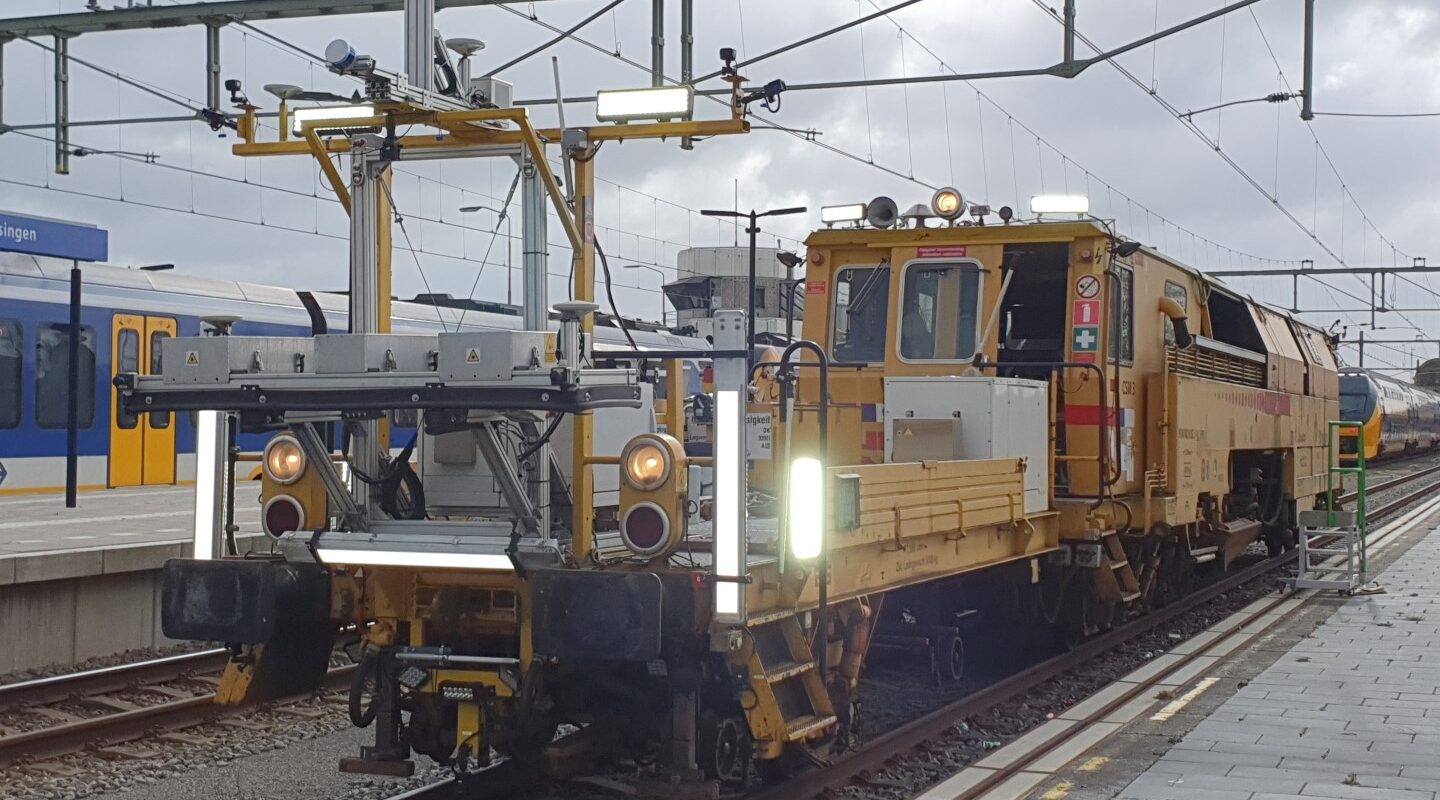
\includegraphics[width=0.7\textwidth]{Chapters/objdet/figures/LeonardoTrain.jpg}};
    \begin{scope}[x={(image.south east)},y={(image.north west)}]
     \draw[color=red,ultra thick] (0.24,0.92) circle [radius=4mm];
     \end{scope}
\end{tikzpicture}
\caption{Leonardo measurement train. Red circle indicates the position of the LiDAR sensor. {\tiny Image by Strukton Rail.}}
\label{fig:objdet:leonardo}
\end{figure}

The Applanix POSPac\textsuperscript{\tiny\textregistered} Mobile Mapping Suite was used to perform the post-processing of the captured data. This post-processing step includes removing redundant data when the train was stationary. It is also used for registering individual captured scenes into a larger scene.

The first dataset was collected on the $14^{th}$ of June 2021 around the Deventer-Twello region, The Netherlands. The  measurement train drove four times back and forth on the same piece of track. Unfortunately, the measurement train did not turn at the end of the section, but instead just drove backwards. This implies that objects are not captured from both directions. Each trip of the measurement train will be referred to as a \emph{run}. In addition to the captured point cloud, the GPS location, heading, acceleration, and odometer of the train are also logged. 

An additional smaller dataset was collected around the city of Dronten, The Netherlands. This trajectory was captured on the $16^{th}$ of November 2021 and consists of a single run.

For both areas, the EPSG:32631 coordinate reference system (CRS) was used for the captured point clouds and for the timestamps Coordinated Universal Time (UTC) was used. The corresponding trajectory logs of the measurement train were recorded using the EPSG:4258 CRS and made use of the Central European Summer Time (CEST,~UTC+02:00) and the Central European Time (CET,~UTC+01:00) respectively. Figure~\ref{fig:objdet:trajectory} shows the trajectory of both measurement sessions.

\begin{figure}[ht]
    \centering
    \begin{subfigure}{0.45\textwidth}
        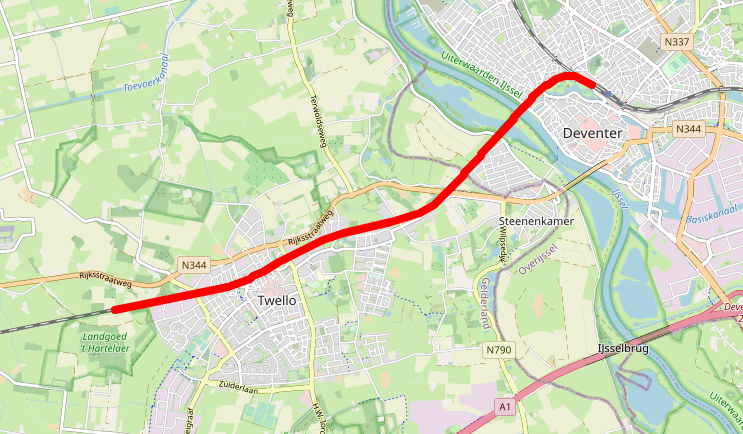
\includegraphics[width=\textwidth]{Chapters/objdet/figures/roi.png}
        \caption{Deventer-Twello area}
    \end{subfigure}%
    \hfill
    \begin{subfigure}{0.45\textwidth}
        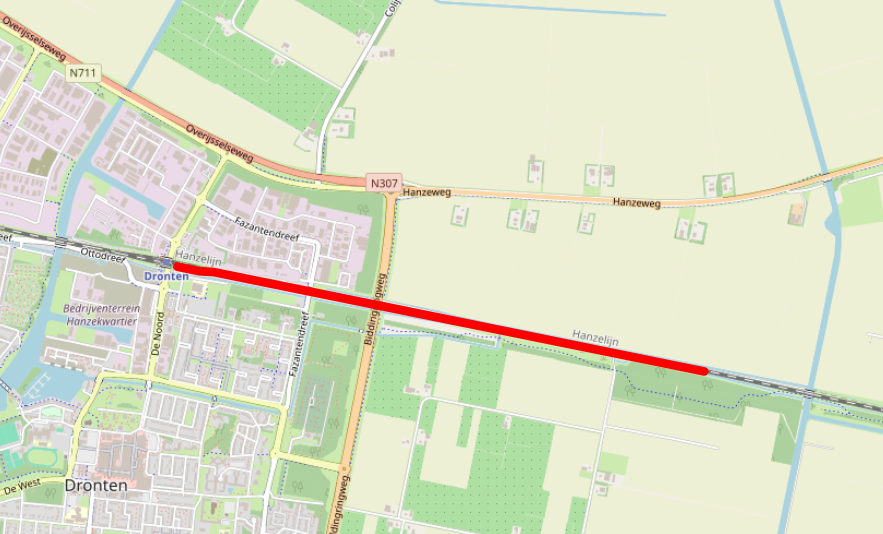
\includegraphics[width=\textwidth]{Chapters/objdet/figures/dronten.png}
        \caption{Dronten area}
    \end{subfigure}%
    \caption{Trajectories of measurement train indicated in red. {\tiny Map data from OpenStreetMap.}}
    \label{fig:objdet:trajectory}
\end{figure}

The average distance of a single run within the Deventer-Twello region was $\approx$6.5~km and the length of the Dronten trajectory was $\approx$2.9~km. The key figures of the different runs are summarised in Table~\ref{tbl:objdet:runstats}. The distance value is based on the odometer data. The table also clearly shows the correlation between the speed and the number of points collected. It can be seen that run~1 had the lowest average speed of 62.4~km/h and the highest point count. Whilst run~4 had the highest average speed of 72.1~km/h and the lowest point count.
\begin{table}[ht]
    \centering
    \begin{tabular}{rllll}
        \toprule
        & Duration [s] & Distance [m] & Speed [km/h] & Points [-]\\
        \midrule
        run 1   & 373.6 & 6476.6 & 62.4 & 59,607,089\\
        run 2   & 325.8 & 6479.3 & 71.6 & 52,834,759\\
        run 3   & 346.4 & 6476.5 & 67.3 & 55,257,052\\
        run 4   & 323.4 & 6479.2 & 72.1 & 52,423,814\\
        dronten & 119.8 & 2867.3 & 86.1 & 16,532,528\\
        \bottomrule
    \end{tabular}
    \caption{Key figures of the different runs and the Dronten test set}
    \label{tbl:objdet:runstats}
\end{table}
The number of points which will be processed will be significantly reduced during the pre-processing steps. To prevent repetitive labelling, all four runs were merged together before the labelling process. To be able to separate the individual runs again after labelling, each point has an additional attribute `run'.

\subsection{Labelling}
Prior to labelling, the large point cloud scene is divided into sections of 250~m long using the same approach described in Section~\ref{sec:objdet:partitioning}. This ensures that the sections are tractable and can be divided amongst multiple people performing the labelling task. As the point density of the scenes is not very high, the fact that labelling is very time-consuming, and given the explorative nature of this research, the following limited set of four object classes are defined: masts, tension rods, signals, and relay cabinets. Figure~\ref{fig:objdet:classes} provides examples of each of the object classes. To provide a scale perspective, an average point cloud human being with a height of 174~cm is plotted alongside the examples. 

Labelling the objects within the point cloud data was done using the open source application CloudCompare. The segment tool was used for drawing polygons around the objects of interest. In general, an unobstructed top view of the object is possible, making it easy to segment the object by drawing a polygon around the object from this view point. After cutting out the object, a label and a unique identifier are added as a `Scalar Field'. Finally all the individual pieces of the dissected scene were merged together again. The unique identifier has proven to be very useful when iterating over each of the individual objects during subsequent processing steps.

The benefit of labelling points instead of just bounding boxes is that the dataset can serve both segmentation and object detection tasks.% Note that the direction of objects is not encoded in the dataset, this is still an issue to be addressed.

\begin{figure}[ht]
    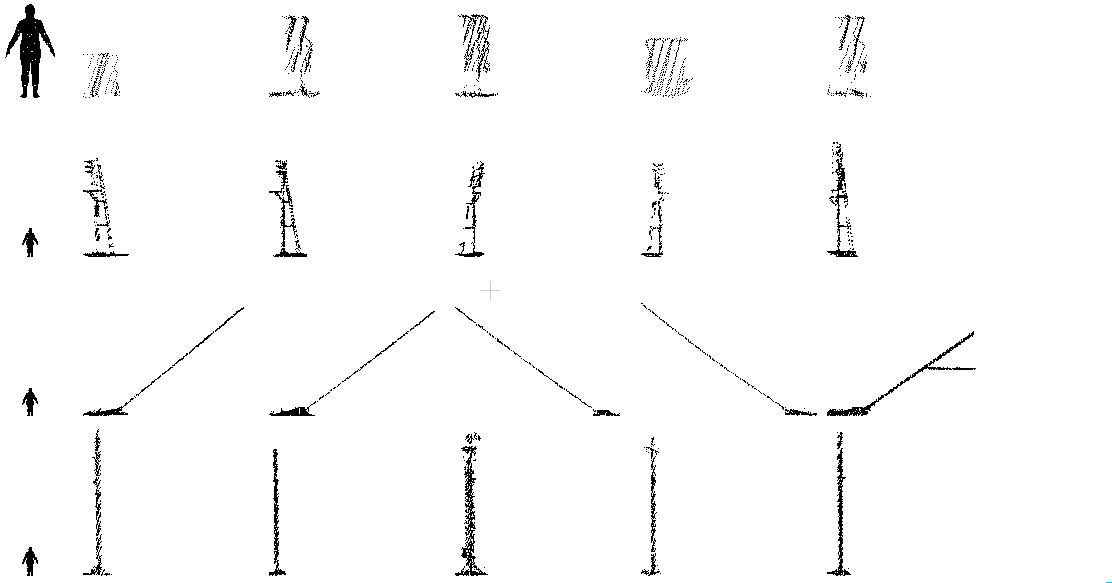
\includegraphics[width=0.9\textwidth]{Chapters/objdet/figures/density_classes2.png}
    \caption{Samples of object classes, From top to bottom: relay cabinet, signal, tension rod, mast. Last three rows are scaled by 0.3. A human being with an average height of 174~cm is added for scale comparison.}
    \label{fig:objdet:classes}
\end{figure}

\subsection{Key figures}
This section provides some key figures of the labelled datasets. Table~\ref{tbl:objdet:stats} shows the class distribution, and the mean and average number of points per object class. It can be seen that the standard deviation of number of points per object is large. This large variation can have several causes, such as the distance between sensor and object, or obstructions between sensor and object.

\begin{table}[ht]
    \centering
    \begin{tabular}{rrrrrrr}
        \toprule
        & \multicolumn{2}{c}{First run} & \multicolumn{2}{c}{Fourth run} & \multicolumn{2}{c}{Dronten}\\
        & Occ. & M (SD) & Occ. & M (SD) & Occ. & M (SD)\\
        \midrule
        Mast &          209 & 992 (516) & 203 & 892 (482) & 124 & 983 (412)\\
        Tension rod &    29 & 710 (395) &  30 & 750 (589) &  24 & 494 (152)\\
        Signal &         20 & 930 (507) &  22 & 810 (400) &   9 & 854 (232)\\
        Relay cabinet &  35 & 392 (175) &  34 & 345 (184) &   2 & 216 (14)\\
        \bottomrule
    \end{tabular}
    \caption{Occurrence (Occ.) of objects and their mean (M) and standard deviation (SD) of point count per object type.}
    \label{tbl:objdet:stats}
\end{table}

The Dronten dataset shows a very low count of relay cabinets. This is attributed to presence of a sound barrier adjacent to large parts of the track. Relay cabinets usually reside on the other side of the sound barrier. This sound barrier obstructs the line-of-sight from the laser scanner resulting into an extremely low count of relay cabinets.

\subsection{Pre-processing}
Before a model can be trained, an elaborate set of pre-processing steps are required to get the data in the right format such that it can be ingested by the model. These steps are described in the following subsections. To ensure that a local object location can be mapped to a real-world location again, it is necessary to keep track of the net transformation during each of the subsequent processing steps.

\begin{figure}[ht]
    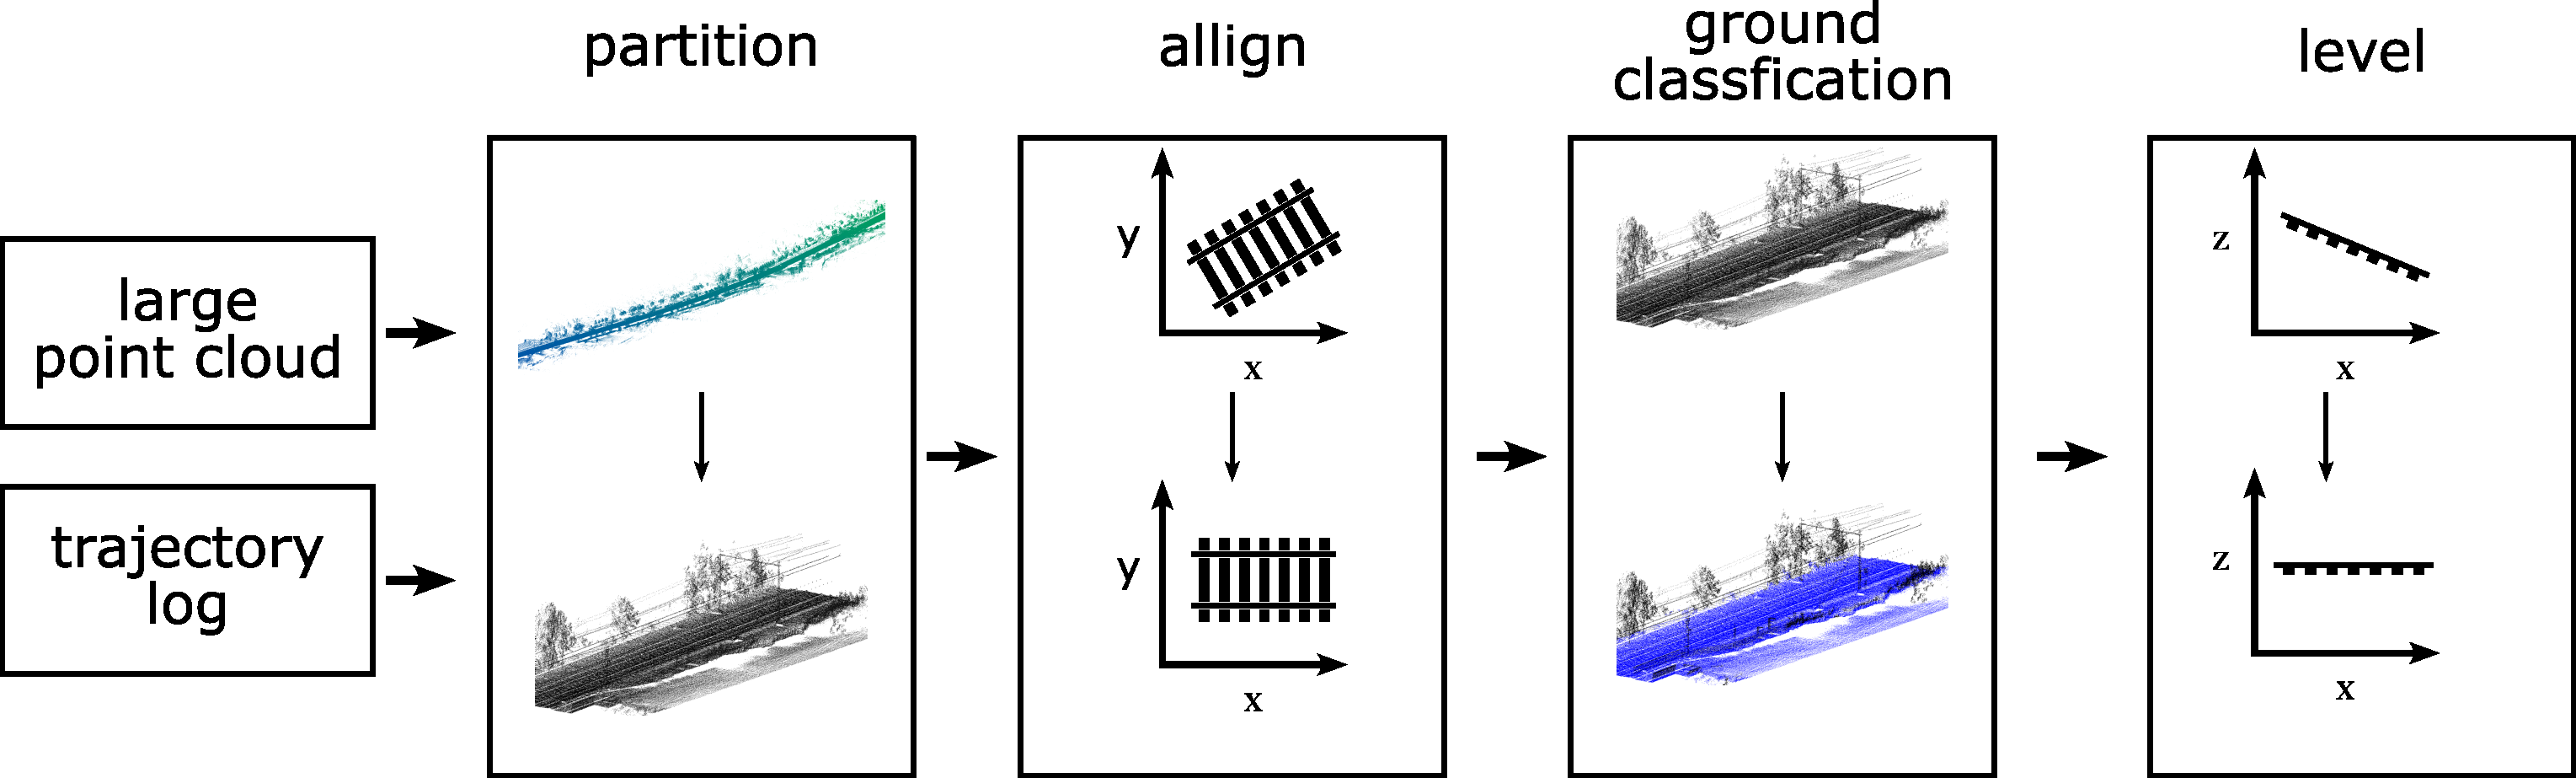
\includegraphics[width=0.9\textwidth]{Chapters/objdet/figures/processing.png}
    \caption{Pre-processing steps.}
    \label{fig:objdet:processing}
\end{figure}

\subsubsection{Partitioning}\label{sec:objdet:partitioning}
The first step in the pre-processing chain is to partition the data into equal length pieces. After the data is collected by the measurement train it is post processed. During this post processing step, the non-stationary `frames' are merged together to form one large point cloud. The frames which are collected when the measurement train is stationary are omitted. To avoid large time gaps in the timestamps of the individual points, the time is shifted to compensate for the omitted frames. Unfortunately this time shift is not reflected in the trajectory log, implying that the timestamps of the point cloud data and the trajectory log are not in sync.

Nonetheless, the trajectory log still plays an important role to define simple polygons which are then used as a cookie cutter to partition the large point cloud scene into smaller tractable pieces. On several occasions, the measurement train drove multiple times on the same track or on an adjacent track. In order to distinguish individual trips, a region of interest can be defined and based on the \(\Delta t\) of the timestamps it is possible to distinguish them. A large \(\Delta t\) means that the measurement left the region of interest and entered it again at a later time instance. A caveat with this approach is that the measurement train cannot change direction within the region of interest.

Based on the timestamps from the trajectory log relating to a single trip, the cookie cutter polygons are defined. This is done by first calculating the cumulative distance based on the odometer data which is present in the trajectory log. Together with the desired length of the pieces, it is possible to determine the locations belonging to the start and end of a piece. These locations will be referred to as \(p_1\) and \(p_2\). To define a cookie cutter polygon, the slope of the line between these two points is determined. Based on this slope it is possible to determine the slope of a line perpendicular to the line passing through the two points (\(p_1\) and \(p_2\)). Given the desired extent of a piece, and the equations of the perpendicular lines it is possible to determine the four vertices of the polygon (\(v_{x,1}, v_{x,2}\) were \(x \in \{1,2\}\)). Figure~\ref{fig:objdet:partitioning} clarifies the procedure. The vertices \(v_{2,1}\) and \(v_{2,2}\) are shared with the next polygon.

\begin{figure}[ht]
    \centering
    % https://www.geogebra.org/m/xr6nVvt4
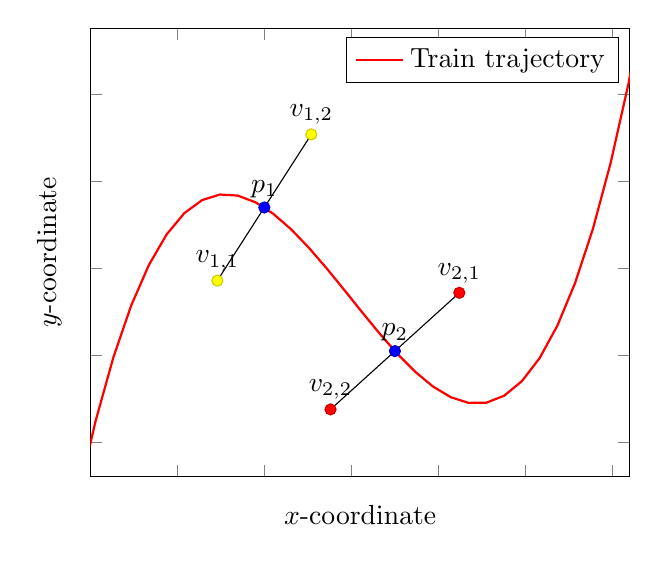
\begin{tikzpicture}
\begin{axis}[
    unit vector ratio=1 1 1,
    xmin=-2, xmax=4.2,
    %ymin=2, ymax=9,
    samples=50, 
    xlabel={$x$-coordinate}, ylabel={$y$-coordinate},
    xticklabels={,,},yticklabels={,,}]
\addplot[
    thick,
    red
] (x, 0.2*x*x*x-0.6 *x *x -0.65 *x + 2.7);
\addlegendentry{Train trajectory}

\addplot[
    scatter,
    mark=*, only marks,
    point meta=\thisrow{color},
    nodes near coords*={\annotvalue},
    visualization depends on={value \thisrow{label} \as \annotvalue},	
] table [] {
   x y color label
   0.00 2.70 1 $p_1$
   1.50 1.05 1 $p_2$
};

\addplot[
    scatter,
    mark=*,
    point meta=\thisrow{color},
    nodes near coords*={\annotvalue},
    visualization depends on={value \thisrow{label} \as \annotvalue},	
] table [] {
   x y color label
    -0.54 1.86 2 $v_{1,1}$
     0.54 3.54 2 $v_{1,2}$
};

\addplot[
    scatter,
    mark=*,
    point meta=\thisrow{color},
    nodes near coords*={\annotvalue},
    visualization depends on={value \thisrow{label} \as \annotvalue},
] table [] {
    x y color label
    2.24 1.72 4 $v_{2,1}$
    0.76 0.38 4 $v_{2,2}$

};

\end{axis}
\end{tikzpicture}
    \caption{Partitioning of the point cloud scene.}
    \label{fig:objdet:partitioning}
\end{figure}

\subsubsection{Alignment}
The two points, \(p_1\) and \(p_2\), from the previous step, which indicate the start and end position of a piece, are used for centring the scene and aligning the track along the \(x\)-axis. First the intermediate point between \(p_1\) and \(p_2\) is determined and is used to set the translational part of an affine transformation. The rotational part of the affine transformation, which aligns the scene alongside the \(x\)-axis, is based on the angle between the \(x\)-axis and the point \(p_1\).

After alignment, the point cloud is clipped in the \(y\)-direction to $[-15~m,15~m]$. Furthermore, a voxel based subsampling method is applied to homogenise the point density. In this scenario a voxel size of 5~cm was used, within each voxel the centroid of the points is calculated. The calculated centroid is used to query the nearest neighbour within the voxel. This nearest neighbour is returned. A grid based subsampling strategy is also used by \citeauthor{grandio2022point}~\cite{grandio2022point}. Density variations occur naturally due to the fact that objects close to the sensor are captured with a higher spatial density compared to objects which are further away.

\subsubsection{Ground classification}
The next step in the pre-processing pipeline is to classify the scene into ground and non-ground points. This classification step serves two purposes, the first purpose is to use the classified ground points to determine a transformation which aligns the scene to the \xyplane{}. The second purpose is to reduce the amount of data being worked with by removing the ground points from the scene during training and inference. The ground classification algorithm used is based on cloth simulation~\cite{csf.16}, result of this classification is stored in the Classification field of the Point Data Record.

The removal of the ground plane is also done by Ariyachandra and Brilakis to reduce computation time and false positives~\cite{ariyachandra2020digital}.

\subsubsection{Levelling}
The least-squares method is used to fit a plane to the classified ground points. The normal vector of this plane is used to determine a rotation matrix which levels the scene and makes it flush with the \xyplane{}. Special care is taken such that the normal of the plane is pointing towards the positive $z$-direction. If this is not the case, the scene would be flipped upside down. Level normalisation is an important prerequisite for the next pre-processing step, determining bounding boxes.

\subsubsection{Bounding boxes}
In general, the task of object detection is to predict (oriented) bounding boxes of objects. This section describes how an oriented bounding box is obtained from a cluster of labelled points. A constraint imposed by the used models is that the top and bottom of the bounding box are flush with the \xyplane{}. An oriented bounding box is represented by a vector with seven elements. These elements are: the centre point of the bounding box ($x,y,z$), the extent in all directions ($ex, ey, ez$) and a yaw angle ($\theta$). The yaw angle is defined as the counter-clockwise rotation around the positive $z$-axis.

The processing steps to determine an oriented bounding box based on point clusters is detailed below:

\begin{itemize}
    \item Determine convex hull of the \(xy\)-coordinates of the cluster.
    \item Use a Singular Value Decomposition (SVD) of the \(xy\)-coordinates of the hull to obtain the orientation of the object.
    \item Rotate the cluster of points such that it aligns with the \(x\)-axis.
    \item Determine the extent (\(ex, ey, ez\)) of the object in \(x, y, z\)-directions.
    \item If \(ey > ex\), swap \(ex\) and \(ey\) and add \(\pi/2\) to the yaw angle.
\end{itemize}

The convex hull of the cluster of points is used to avoid point density variations altering the true orientation of the bounding box when the SVD is applied in the next step. The final step ensures that the longest side of the bounding box is always aligned with the \(x\)-axis. This is important when calculating the dimensions of the anchor boxes, otherwise the dimensions of the anchor boxes would be distorted. Figure~\ref{fig:objdet:sample} shows a sample scene. It shows the labelled points and the calculated bounding boxes.

\begin{figure}[ht]
    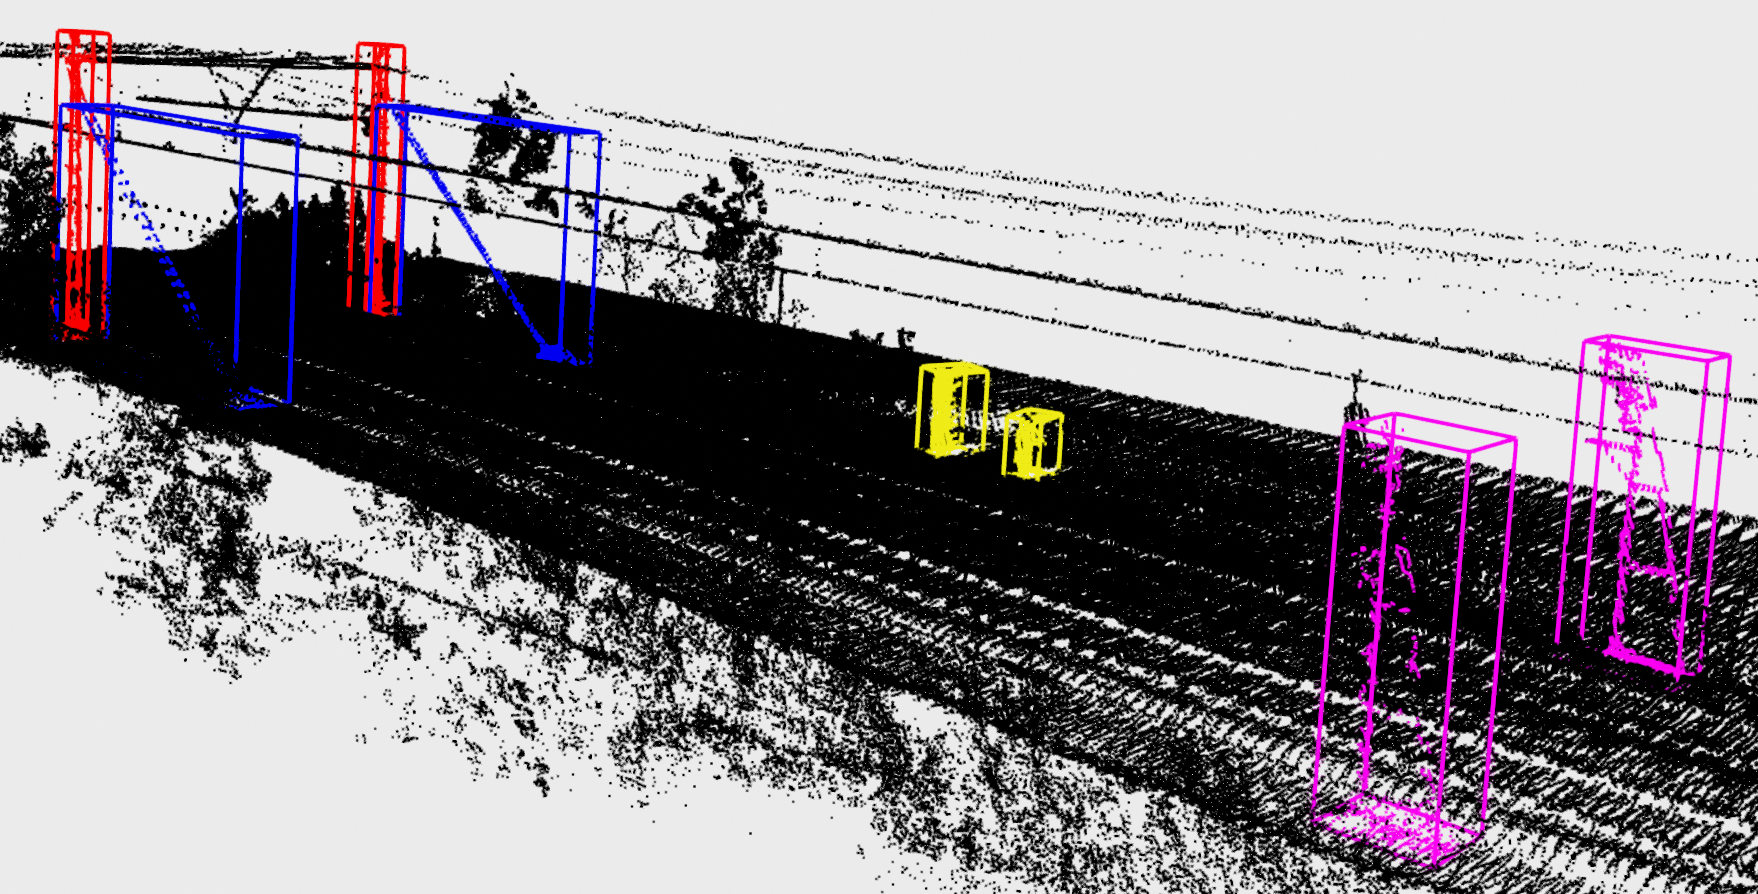
\includegraphics[width=0.9\textwidth]{Chapters/objdet/figures/run1_scene11.png}
    \caption{Sample scene. Red: masts, blue: tension rods, magenta: signals, yellow: relay cabinets, and black: background. Labelled points and calculated bounding boxes are visible. Best viewed in colour.}
    \label{fig:objdet:sample}
\end{figure}

\textbf{Anchor box statistics}\\
The PointPillar model requires an initial estimate of the bounding box sizes of the objects of interests. These estimates are referred to as anchor boxes. The anchor box dimensions are summarised in Table~\ref{tbl:objdet:abstats}.

\begin{table}[ht]
    \centering
    \begin{tabular}{rrrr}
        \toprule
         & width & length & height\\
        \midrule
        Mast & 1.4 & 1.1 & 8.9\\
        Tension rod & 10.6 & 1.2 & 7.1\\
        Signal & 2.4 & 1.3 & 6.2 \\
        Relay cabinet & 1.5 & 0.8 & 1.6 \\
        \bottomrule
    \end{tabular}
    \caption{Dimensions (m) of the anchor boxes of the first run per object class.}
    \label{tbl:objdet:abstats}
\end{table}

\section{Methodology}
Two successful deep learning based 3D object detection models, the PointPillar model (2019)~\cite{pointpillar} and the CenterPoint model (2021)~\cite{centerpoint}, from the domain of autonomous driving will be evaluated for the task of detecting objects within the railway environment. The PointPillar and CenterPoint object detection models are chosen for this application as they have good performance in terms of average precision and have a low inference time making it suitable for practical applications~\cite{guo2020deep}. The CenterPoint model supports both a pillar based discretisation and a voxel based discretisation of the scene. In this work, to ensure a fair comparison between both models, the pillar based discretisation is used.

Both models utilise the SECOND backbone~\cite{second18}, which is an improved version of the VoxelNet backbone~\cite{voxelnet18}. The main difference between the two models is the type of head. The CenterPoint model uses a two-stage approach. First the centre of the object is located (hence the name). Secondly, a regression head is used to predict the bounding box and orientation. This also implies that no prior information about the box sizes in the form of anchor boxes is required. The PointPillar model on the other hand uses a Single Shot Detector (SSD) to estimate bounding boxes in the 2D Birds Eye View (BEV). The 3D bounding box height and elevation are additional regression targets. The original CenterPoint model has the velocity as a regression output as well. Though, for this study, the velocity regression target has been omitted from the model.

The grid size used by the original CenterPoint model is $(0.2\times 0.2~m)$ or $(0.32\times 0.32~m)$, depending on the dataset being evaluated. The grid size used by the original PointPillar mode is $(0.16\times 0.16~m)$. In an ablation study, the authors of the PointPillar model show that the performance diminishes as the grid size increases. Therefore, for this study a grid size of  $\approx (0.1\times 0.1~m)$ has been used. This grid size has been chosen as a good balance between locational accuracy and memory consumption of the model. The resulting grid size was \(736\times 304\).

\subsection{Evaluation method}
All possible permutations for training, validation and testing are evaluated on the four runs of the Deventer-Twello dataset. This means that in total $4! = 24$ experiments are conducted. The model which performs best on the validation set is used for testing. The mean average precision (mAP) specified at an Intersection over Union (IoU) threshold of 0.5 and 0.75 are used as final metric. The results of all permutations are averaged and presented with the standard deviation.

The software framework used for evaluating the model is non-deterministic. Hence, to reduce the variability of the validation and test results, the validation and testing datasets are iterated ten times when determining the AP values.

As there is no standardised definition of calculating the mAP, the details of the calculation are provided here. The metric used in this work could be considered a vanilla type of mAP. When determining the precision and recall values, the confidence threshold is varied. In our work all encountered prediction certainty scores are used as confidence threshold values. The IoU values are volume based.

In addition to the overall average precision scores, the impact of point count for the mast class is also evaluated. This class has been chosen as it is the most common class in the dataset. To evaluate the impact, the masts have been divided into four quantiles based on point count. For each quantile the recall curve is determined, the precision recall is not considered, as it would be impossible to determine to which quantile a \emph{False Positive} will contribute. For each confidence threshold the recall (Equation~\ref{eq:objdet:recall}) is calculated, in this equation $TP$ refers to the number of \emph{True Positive}s and $FN$ refers to the number of \emph{False Negative}s. The IoU threshold is set to 0.5.

\begin{equation}
    Recall = \frac{TP}{TP + FN} 
    \label{eq:objdet:recall}
\end{equation}

The final metric reported will be the Area Under Recall Curve (AUReC).


\subsection{Transfer learning}
Labelling data is an expensive endeavour, therefore it is valuable to know how much effort is required to get good results from an unseen, new piece of track. Transfer learning is a successful technique to make use of an existing trained model and fine tune it for a new data~\cite{razavian14,tajbakhsh16}.

The Dronten dataset is used to get insights into how much new training is required to obtain good results. The dataset is manually split into four distinct subsets were care is taken that the distribution of classes is roughly equal amongst these subsets. 

The amount of new training data is varied, by taking 0\%, 25\%, 50\%, and 75\% of the Dronten dataset. The remaining data is used for testing. As there are very few examples of relay cabinets present in this dataset, this class if omitted for this experiment. As the dataset is too small to also have a proper validation set, the number of training epochs is fixed to 600. The learning rate is set to $1\times 10^{-4}$. The reported metric will be the mAP of the test set based on the weights of epoch 600.

The number of possible permutations of training and testing sets for the case of 25\% and 75\% is four. For the case of 50\% training data, the number of permutations is twelve. All permutations are trained and evaluated, and the average mAP is reported. An initial single model is trained on the Deventer-Twello dataset with the relay cabinet class ignored. This initial model is then fine tuned using varying amount of training data from the Dronten dataset.

\subsection{Locational error}\label{sec:objdet:obserr}
The locational error between the ground truth location and the location predicted by the machine learning models can be decomposed into two components, the random error and the systematic error~\cite{regtien}. We will adhere to the terminology set out by the ISO~5725-1 standard~\cite{iso5725}. This standard introduces the concept of trueness, which captures the systematical error and precision, which captures the random error. Both error components combined constitute the accuracy. The errors are analysed for the masts and cabinets together with an overall analysis. The other two asset classes, tension rods and signals are not considered as it is not possible to define a precise origin for these two classes. For instance, in our case the tension rods have been labelled together with their concrete foundation, whilst the reference data only labelled the rods themselves. A similar case holds for the signals, in our case signals have been labelled together with the attached staircase, whilst the reference data did not.

Evaluation of the locational accuracy of the assets detected by the machine learning model requires accurate ground truth data. Often this data is not available as it requires considerable resources to obtain this data, especially for longer stretches of track. As an alternative, the Dutch railway manager ProRail provides the absolute location of a large number of railway assets situated in the Netherlands. The locations of selected assets are publicly made available using a Web Feature Service (WFS)~\footnote{https://mapservices.prorail.nl} which can be queried. It is not known how these locations are obtained, but it is most likely done using photogrammetry, and what the expected accuracy of these locations is. Hence, the first step will be to evaluate the locational accuracy of the data provided by ProRail.

To do so, a geodetic survey was carried out using a Leica~GS18 GNSS RTK rover during the night of 28--29$^{th}$ January 2024. The data sheet of this rover lists a mean horizontal accuracy of 7~mm and a mean vertical accuracy of 25~mm. 74 objects (4 signals, 12 catenary rods and 58 masts) were surveyed and compared to the dataset provided by ProRail. The masts were all steel H-profile style masts, the centre of the H on the ground plate has been used as measurement point. Based on mast locations, it was concluded that all objects surveyed fall within a locational accuracy of 10 centimetres horizontal ($\mu$ 8.7~cm, $\sigma$ 4.5~cm with a maximum error of 19.6~cm). Therefore, we consider the locations provided by ProRail a valid proxy source for the ground truth.

This ProRail data is then used to evaluate the locational accuracy of the detected objects. The criteria for a detected object to be included in the evaluation was if the detected the object was within 3 metres of the location specified by ProRail and the detected object had the correct label. Otherwise, the detection was excluded. In order to get meaningful results when comparing locations of objects, both datasets must use the same origin. For the catenary masts and cabinets the horizontal position of the origin is set to the centre of these objects. The ProRail data does not include the vertical position (z-component). Therefore the decision was made to only include the horizontal components in the evaluation of the locational accuracy.

The locational error is analysed for the mast and cabinet asset classes. For each asset class there are $n_{gt}$ ground truth locations, for each ground truth location there are $n_{d,i}$ detections from the models. In total for a certain asset class there will be $n_d$ detections. Let $p_i$ be a vector denoting a specific ground truth location, where $i$ is an index over the number of ground truth locations for this asset class. Let $\tilde{p}_{i,j}$ be another vector, specifying a certain detection corresponding to a ground truth location $i$, and $j$ is an index over the number of detections for this ground truth location.

\subsubsection{Trueness} % Systematic error, aka bias (formerly known as accuracy)
To determine the trueness, the systematic error vector $\delta$ can be determined based on the difference between the ground truth locations and the detections from the machine learning models. Equation~\ref{eq:objdet:syserr} shows how this systematic error vector is formally defined.

\begin{equation}
   \delta = \frac{1}{n_d} \sum_{i=1}^{n_{gt}} \sum_{j=1}^{n_{d,i}} \tilde{p}_{i,j} - p_i
   \label{eq:objdet:syserr}
\end{equation}

The trueness for an asset class is defined as the norm of the systematic error vector, that is $||\delta||$.

\subsubsection{Precision} % Random error
The precision of the detections will be represented by the standard deviation of the measurements. The standard deviation will be represented by a vector $\sigma$, consisting of the elements $\sigma_x$ and $\sigma_y$. As an example, the calculations for determining the standard deviation $\sigma_x$ are provided, $\sigma_y$ is derived in the same way. To determine the standard deviation $\sigma_x$ of the detections corresponding to a ground truth location $p_i$, first the arithmetic mean $\tilde{\mu_i}$ of the detections $\tilde{p}_{i,j}$ is determined. Thereafter, Equation~\ref{eq:objdet:precision} shows how this mean value is used to determine the precision. 

\begin{equation}
    \sigma_x = \frac{1}{n_{gt}} \sum_{i=1}^{n_{gt}} \sqrt{\frac{\sum_{j=1}^{n_{d,i}} (\tilde{p}_{{i,j}_x} - \tilde{\mu_{i_x}})^2}{n_{d,i}}}
    \label{eq:objdet:precision}
\end{equation}
The overall precision is defined as $||\sigma||$.

\subsubsection{Accuracy} % Combi van trueness en random error
The overall locational accuracy for a certain asset class will be measured using the Root Mean Square Error (RMSE) vector. This metric encompasses both trueness and precision. The RMSE vector for a single ground truth location $i$ is composed of the individual $m_{i_x}$ and $m_{i_y}$ components. Equation~\ref{eq:objdet:Mx} shows how the $m_{i_x}$ component is calculated. The other component is calculated in similar fashion.

\begin{equation}
    m_{i_x} = \sqrt{\frac{1}{n_{d,i}} \sum_{j=1}^{n_{d,i}} (\tilde{p}_{{i,j}_x} - p_{i_x})^2}
    \label{eq:objdet:Mx}
\end{equation}

Finally, the RMSE can be calculated using Equation~\ref{eq:objdet:rmse}. 
\begin{equation}
    RMSE_i = \sqrt{m_{i_x}^2 + m_{i_y}^2}
    \label{eq:objdet:rmse}
\end{equation}
The reported RMSE for a certain asset class will be the average of all RMSE values belonging to this asset class.

\subsection{Training setup}
Due to memory consumption of the model during training, a batch size of one is used. Initially the model had difficulty converging, this is why for training a Stochastic Gradient Descent (SGD) optimiser is used instead of the default Adam optimiser. SGD provides a better generalisation, with the penalty of having a slower training time~\cite{ZhouPan20}. A total of 3000 epochs are trained, with an initial learning rate of $1\times 10^{-3}$ and after 1500 epochs this is reduced to $1\times 10^{-4}$. Every 50 epochs, the model is validated and the weights corresponding to the highest mAP of the validation set are retained. These model weights are later used for testing.  

The models are trained on a desktop computer with 64~GB of RAM, an AMD Ryzen Threadripper 2950X CPU, and an NVIDIA TITAN~V GPU with 12~GB of memory.

\section{Results}
First, the object detection results are presented in terms of average precision. In addition, the impact of point density on the recall rate of the catenary masts is presented. Thereafter, the effectiveness of transfer learning is analysed. Because accurate locational information is essential when creating `as-is' models, an in depth analysis of the locational error is provided. Finally, two rejected hypotheses are presented for completeness.

\subsection{Object detection}
The aggregated object detection results are presented in Table~\ref{tbl:objdet:mAP}. The table shows the average precision results averaged across the different experiments together with the standard deviation.

\begin{table}[ht]
    \centering
    \begin{tabular}{rllll}
        \toprule
        & \multicolumn{2}{c}{$IoU \ge 0.5$} & \multicolumn{2}{c}{$IoU \ge 0.75$}\\
        \cmidrule(lr){2-3} \cmidrule(lr){4-5}
        Asset & PointPillar & CenterPoint & PointPillar & CenterPoint\\
        \midrule
        Mast &          78.5 (11.1) & 72.8 ( 8.5) & 16.3  (9.6) &  7.5 (4.1)\\
        Tension rod &   71.7 (11.9) & 64.3 (14.1) & 12.6  (8.7) &  9.7 (4.8)\\
        Signal &        83.5 ( 7.0) & 82.1 ( 7.0) & 16.3 (11.3) & 14.0 (6.5)\\
        Relay cabinet & 48.6 (11.5) & 36.3 (13.1) &  2.4  (2.5) &  0.5 (1.2)\\
        \midrule
        \textit{mAP}  & 70.6 (8.0) & 63.9 ( 6.8) & 14.6 (15.1) & 10.3 (11.8)\\
        \bottomrule
    \end{tabular}
    \caption{Mean AP@0.5 and AP@0.75 results for all combinations of training, validation, and testing. Standard deviation in brackets.}
    \label{tbl:objdet:mAP}
\end{table}

From the table it can be seen that the performance quickly degrades when an IoU threshold of 0.75 is used. This is already an indication of poor locational accuracy as the IoU directly depends on how well bounding boxes overlap. An in depth analysis of the locational accuracy is provided in Section~\ref{sec:objdet:obserr}. The table also shows that the PointPillar model has the best performance for all classes, albeit with a slightly higher standard deviation. 

The results of determining the impact of point count on the recall rate are provided in Table~\ref{tbl:objdet:quantile}. The first and last quantile show the largest spread in point count. The samples column specifies the number of samples falling within the listed interval.

\begin{table}[ht]
    \centering
    \begin{tabular}{rlll}
        \toprule
        Quantile & Interval & Samples & AUReC\\
        \midrule
        1 & [ 159, \space 629) & 212 & 58.9 (11.2)\\
        2 & [ 629, \space 783) & 210 & 67.5 (11.3) \\
        3 & [ 783, 1076)       & 214 & 62.8 ( 9.3)\\
        4 & [1076, 4486]       & 212 & 63.8 ( 7.4)\\
        \bottomrule
    \end{tabular}
    \caption{Area Under Recall Curve (AUReC) for each quantile for the masts using an IoU threshold of 0.5.}
    \label{tbl:objdet:quantile}
\end{table}

Surprisingly, the data does not show a positive correlation between point count and the AUReC. This was expected as a higher point count would also imply more information to be present for the machine learning model to learn on.

\subsection{Transfer learning}
The results of the transfer learning experiments are presented in Table~\ref{tbl:objdet:transfer}. It should be noted that the results mentioned for the signal class are very imprecise, as the number of signals per split was very limited (1,2,2,4). 

\begin{table}[ht]
    \centering
    \begin{tabular}{rrrrrrrrr}
        \toprule
         & \multicolumn{4}{c}{No TL} & \multicolumn{4}{c}{With TL}\\
         \cmidrule(lr){2-5} \cmidrule(lr){6-9}
         & 0\% & 25\% & 50\% & 75\% & 0\% & 25\% & 50\% & 75\%\\
        \midrule
        Mast &        -- & 70.3 & 84.3 & 82.5 & 57.0 & 86.3 & 90.0 & 91.5\\
        Tension rod & -- &  9.5 & 42.4 & 60.0 & 21.0 & 70.8 & 71.8 & 74.3\\
        Signal &      -- &  8.5 &  6.8 & 12.5 &  6.0 &  6.8 & 19.3 & 12.5\\
        \bottomrule
    \end{tabular}
    \caption{With and without Transfer Learning (TL) for varying amounts of training data. AP@IoU=0.5.}
    \label{tbl:objdet:transfer}
\end{table}

The table shows a clear benefit when using transfer learning. For instance, when using 25\% of the training data the AP for the tension rod class jumps from 9.5\% to 70.8\%.

\subsection{Locational error}
The object detection experiments led to a combined total of 11.761 detections made. From these detections, 1957 detections were excluded from the test resulting in 9804 detections available for analysis. 

First, the locational trueness and precision of the objects detected by the machine learning model are presented. Secondly, the locational accuracy values are presented based on the RMSE.

\subsubsection{Trueness}
The results of the trueness analysis can be found in Table~\ref{tbl:objdet:trueness}. The various experiments of both the PointPillar and the CenterPoint models showed similar results for each object.

\begin{table}[ht]
    \centering
    \begin{tabular}{rrrrrrr}
        \toprule
        & \multicolumn{3}{c}{PointPillar} & \multicolumn{3}{c}{CenterPoint}\\
        \cmidrule(lr){2-4} \cmidrule(lr){5-7}
        Object & $\delta_x$ & $\delta_y$ & $||\delta||$ & $\delta_x$ & $\delta_y$ & $||\delta||$ \\
        \midrule
        Mast & 3.41 & 7.56 & 8.30 & 3.08 & 7.30 & 7.92 \\
        Relay cabinet & 4.73 & 9.59 & 10.69 & 4.83 & 10.86 & 11.88 \\
        \midrule
        \textit{Overall} & 3.56 & 7.79 & 8.56 & 3.27 & 7.70 & 8.36 \\
        \bottomrule
    \end{tabular}
    \caption{Locational trueness analysis (centimetres)} % Sys. fout
    \label{tbl:objdet:trueness}
\end{table}

\subsubsection{Precision}
The results of the locational precision can be found in Table~\ref{tbl:objdet:locpre}. Again, the various experiments of both the PointPillar and the CenterPoint models showed similar results for each object. The precision values fall almost completely within the accuracy of the fixed marks used for comparison. 

\begin{table}[ht]
    \centering
    \begin{tabular}{rrrrrrr}
        \toprule
        & \multicolumn{3}{c}{PointPillar} & \multicolumn{3}{c}{CenterPoint}\\
        \cmidrule(lr){2-4} \cmidrule(lr){5-7}
        Object & $\sigma_x$ & $\sigma_y$ & $||\sigma||$ & $\sigma_x$ & $\sigma_y$ & $||\sigma||$\\
        \midrule
        Mast & 10.35 & 11.97 & 15.83 & 9.49 & 10.07 & 13.83 \\
        Relay cabinet & 17.28 & 12.08 & 21.09 & 24.57 & 11.85 & 27.28 \\
        \midrule
        \textit{Overall} & 11.33 & 11.98 & 16.49 & 12.14 & 10.28 & 15.90 \\
        \bottomrule
    \end{tabular}
    \caption{Locational precision analysis (centimetres)} % Random fout
    \label{tbl:objdet:locpre}
\end{table}

\subsubsection{Accuracy}
The results of the locational accuracy can be found in Table~\ref{tbl:objdet:locacc}.
\begin{table}[ht]
    \centering
    \begin{tabular}{rrrrrrr}
        \toprule
        & \multicolumn{3}{c}{PointPillar} & \multicolumn{3}{c}{CenterPoint}\\
        \cmidrule(lr){2-4} \cmidrule(lr){5-7}
        Object & $m_x$ & $m_y$ & RMSE & $m_x$ & $m_y$ & RMSE \\
        \midrule
        Mast & 15.06 & 20.80 &  25.68 & 14.85 & 19.53 & 24.52 \\
        Relay cabinet & 19.35 & 18.11 & 26.50 & 26.80 & 19.25 & 32.99 \\
        \midrule
        \textit{Overall} & 15.50 & 20.52 & 25.78 & 16.60 & 19.50 & 25.61 \\
        \bottomrule
    \end{tabular}
    \caption{Locational accuracy analysis (centimetres)} % Sys. + random fout
    \label{tbl:objdet:locacc}
\end{table}

In general, the overall locational accuracy is not yet within what is required for (automated) engineering applications. From the results it can be seen that the random error (precision) has the largest contribution to the overall accuracy. Since it is a random error, it should be possible to mitigate this by averaging multiple measurements. There are several possible factors influencing the accuracy. First is the grid size, the finer the grid, the more accurate a location can be determined. Second is the net transform, this net transform is used to map from a local coordinate system back to the global coordinate reference system. Any errors in keeping track of the net transform will be reflected in the locational accuracy. Another possible error cause are the conversions between different coordinate reference systems. Lastly, the accuracy of the GPS system of the measurement train and the post processing steps involved will also impact the locational accuracy. 

\subsection{Rejected hypotheses}
For the sake of completeness and to combat positive-results bias, this section will detail two approaches which were attempted, but were not fruitful in the long run. The first approach relates to an alternative and a more recent object detection algorithm, the second approach relates to semantic segmentation of point cloud data.

\subsubsection{DSVT model}
The Dynamic Sparse Voxel Transformer (DSVT) is a more recent model~\cite{dsvt} which was published in 2023 compared to the PointPillar model which was published in 2019. On paper this model has better results compared to the PointPillar model, an mAP of 79.5 versus an mAP of 69.0 for the Waymo dataset~\cite{waymo}. The hypothesis here was, ``if this newer model has a higher mAP on the benchmark dataset, surely it will also perform better on our own data''. Despite a grid search for optimal hyper-parameters, it was not possible to surpass the 0.5~mAP threshold for our custom rail scene dataset. The reason for this is not known. It could be related to the implementation of the model or still a bad choice of hyper-parameters.

\subsubsection{Semantic segmentation}
During experimentation the realisation was made that object detection based localisation of railway assets does not provide the required locational accuracy. This is caused by the fact that most object detections models are grid-based, labelling inaccuracies exist, and the low tightness of the predicted bounding boxes. To completely overcome the localisation accuracy dependency on grid size, an attempt was made to use a segmentation based model. Based on the fact that semantic segmentation provides a label per point and is not grid-based, the hypothesis was that with some post-processing the location accuracy of objects should be significantly higher. An additional envisioned benefit of segmentation based models is that also `continuous' objects such as tracks and wires can be classified with the same model.

To try this hypothesis in practice, an initial experiment was conducted with the \pnpp{} model to semantically segment the railway scene. The task was to segment the point cloud into the following individual classes: background, mast, signal, tension rod and cabinet. Quickly it was realised that this approach would not be fruitful as the background class accounts for 98\% of the dataset.

\section{Conclusion}
This study has looked at large scale object detection based on point cloud data for the railway environment. These object detections are required to create `as-is' models, which can then be used for a large range of applications. Two deep learning models from the domain of autonomous vehicles have been evaluated for object detection from point cloud data. An overall mAP@0.5 of 70.6\% has been achieved for our custom dataset using the PointPillar model. This custom dataset has been collected for this study as there is a lack of large public (benchmark) datasets for the rail domain.

A limitation of this study, caused by the small custom dataset, is that the main results only present how well the models generalise to repeated measurements. Based on an additional smaller custom dataset, it can be concluded that the models do not generalise well to new railway environments. To overcome this, this research has shown that transfer learning is a viable approach to quickly adapt existing models to new railway scenarios. As an example, when using 25\% of the new training data the AP for the tension rod class jumps from 9.5\% (no transfer learning) to 70.8\% (with transfer learning).

Furthermore, this study has done an in depth analysis of the locational error, which is defined as the difference between the ground truth location and the location of objects estimated by the model. Based on this analysis, it is concluded that the required $\pm$5~cm level of accuracy can not be achieved yet. This analysis decomposed the accuracy into a systematic component and a random component. The random error had the largest contribution to the overall error. Both models showed similar results for the locational error.



\subsection{Recommendations}
For tasks related to autonomous driving there are many large annotated public point cloud datasets available~\cite{YinBerger17}. For tasks related to the railway environment, there were no large public dataset available at the time this study was initiated. Very recent, in 2023/2024 some public datasets related to the rail domain have been published~\cite{dataKharroubi,osdar23,whuRail3D}. It is recommended to utilise these new datasets and evaluated the performance. As these datasets are from very diverse geographic regions, they automatically provide a large variation of object types.

An alternative cost-effective approach to obtain labelled data is to use synthetic data. For instance, the work of Neri and Battisti create a full virtual environment of the railway and use a virtual laser scanner to generate data~\cite{Neri22}. To create a more realistic synthesised scene, the work of Uggla and Horemuz use a hybrid approach were real data and purely synthetic data are combined to create artificial point clouds of railroad level crossings~\cite{uggla2021towards}.

Obtaining sufficient high quality annotations for point cloud data is an expensive task. To alleviate this issue, self-supervised pre-training of the model can be used. A pre-trained model requires less labelled data to achieve similar performances compared to models which are trained from scratch with large amounts of labelled data. A common method of self-supervised learning is contrastive learning, this approach is used by \citeauthor{depthcontrast21} on point cloud data with good results~\cite{depthcontrast21}. It is recommended to also evaluate this approach for the rail domain.

In the case of autonomous vehicles, the deep-learning model consumes frames one-by-one from the laser scanner. A frame consists of all the points collected during a single rotation of the laser scanner. An advantage of this frame data is that it is always relative to the position of the sensor. This is very useful for autonomous driving, because we want to know the location of objects such as other cars, cyclists and pedestrian relative to the car. Unfortunately, in our case it was not possible to obtain the raw frame-by-frame point cloud data. Hence, extensive pre-processing operations were required to split large point clouds into tractable pieces and normalise it such that the data can be ingested by the models. Since the majority of object detection models are developed with autonomous driving in mind, most of these models consume a single frame as input. It would be worthwhile researching to see if better results for the railway environment can be achieved by using frame-by-frame data as input source.

Object detection models aimed at the domain of autonomous vehicles prioritise inference speed and collision avoidance over positional accuracy. To address this issue two approaches are possible. First, an alternative paradigm of object detection models can be explored. Second, additional post-processing steps can be added to the pipeline to increase the locational accuracy. 

Currently a vanilla-style mAP metric was used to evaluate the performance of the models. Recently the nuScenes detection score~\cite{nuscenes20} (NDS) has gained traction. This metric normalises for the fact that objects closer to the sensor are captured with a higher density compared to objects further away from the sensor. The metric also accounts for the size of objects. It is advised to also mention this metric in future work.

The quantiles which were defined to analyse the impact of point density on the recall rate of catenary masts were based on equal group size. Alternative ways to define these quantiles, and the impact thereof, can be explored.

The current work does not add overlap when partitioning the data into tractable pieces. It is expected that adding overlap will lead to a better utilisation of the labelled data, circumventing the issue of objects being split when they reside on the boundaries of the cut.

\clearpage
\printbibliography[heading=subbibnumbered]